\chapter{Introduction (Draft)}

\graphicspath{{../img/ch10/}}
\section{Introduction}

The vast amount of information on the web increases the need of automated processing. Machine processing and machine understanding of textual information is especially difficult. 


Figure~\ref{img:ExtractionProcessIntro} learning and annotation process in general (ILP version later, Chapter~\ref{ch:ILP_Learning})

\begin{figure}
\centering
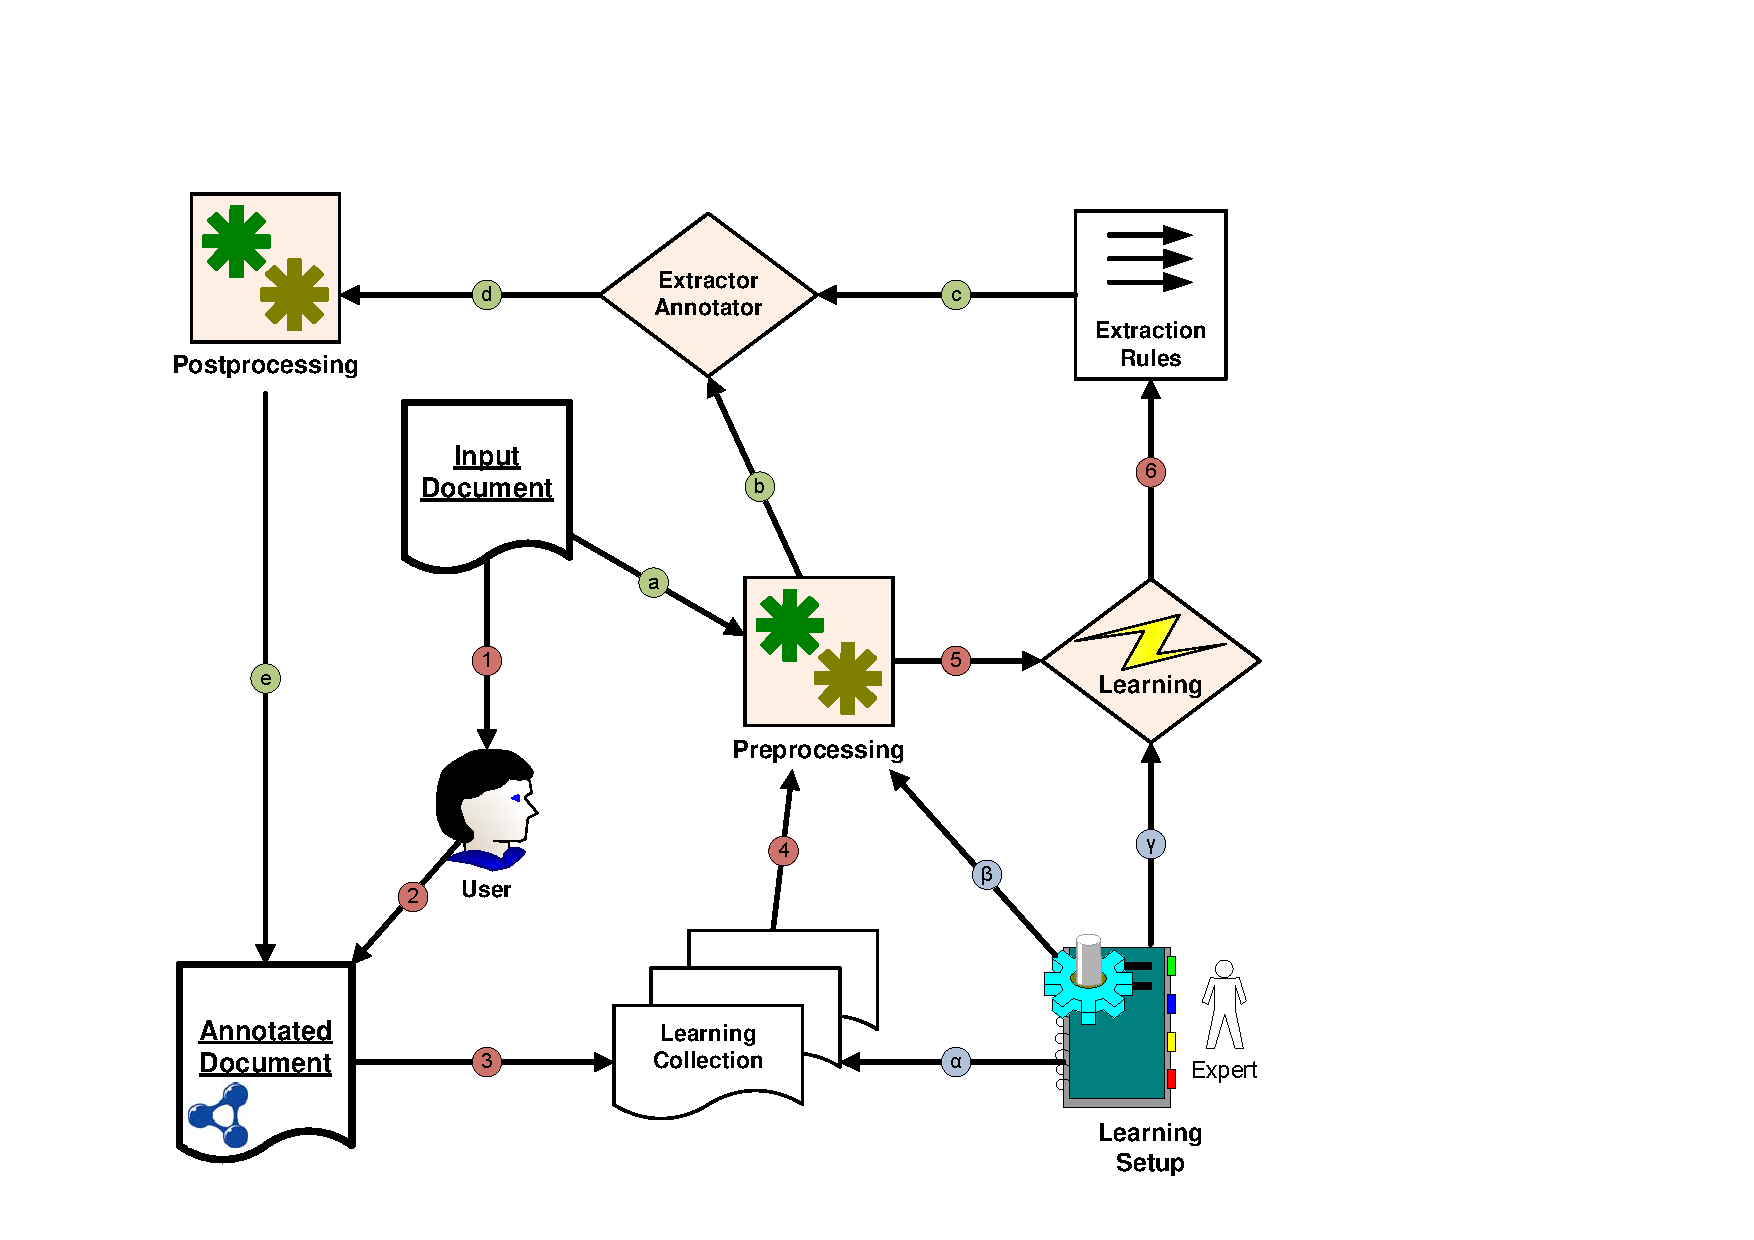
\includegraphics[angle=-90, width=0.8\hsize]{annotation_process}
\caption{Learning and annotation process -- general overview}
\label{img:ExtractionProcessIntro}
\end{figure}


\begin{figure}
\centering
\framebox{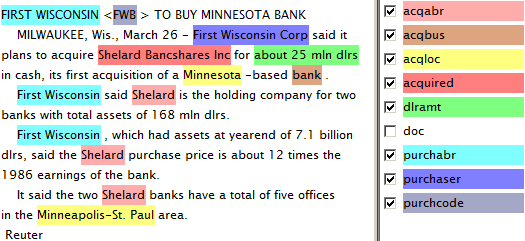
\includegraphics[width=0.7\hsize]{acquisitions_annotated}}
\caption{Corporate Acquisition Events annotations}
\label{img:acquisitions_annotated}
\end{figure}


\begin{figure}
\centering
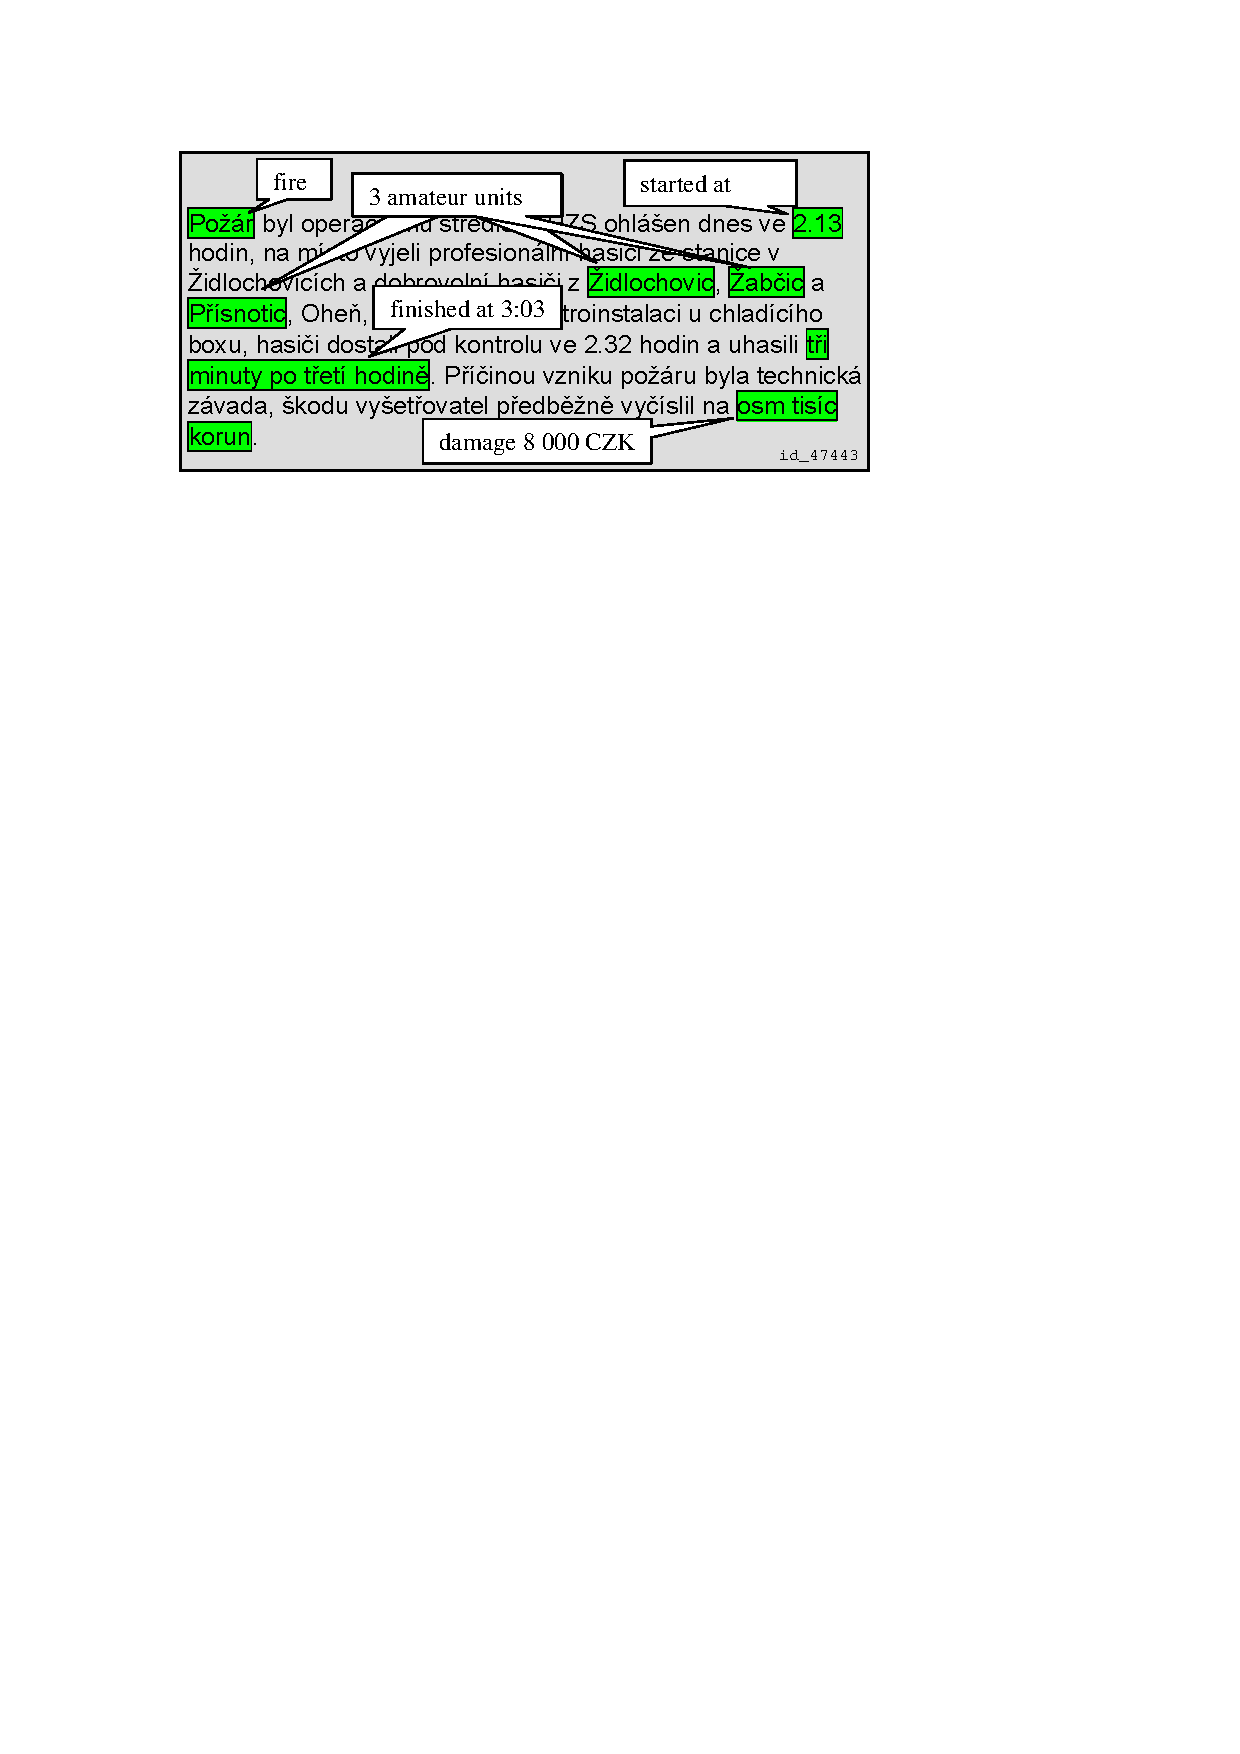
\includegraphics[width=0.5\hsize]{fireman_annotated}
\caption{Fireman Events annotations}
\label{img:fireman_annotated}
\end{figure}


In Figure~\ref{img:ch10_damage_tree}, nodes of the tectogrammatical tree are decorated. A piece of information about the damage of 8000 CZK can be found there (the three nodes on the right). We have used ILP to learn rules that are able to detect these nodes. 

The extraction process requires human assistance when annotating the training data.

Note that our method is general and is not limited to Czech. It can be used with any structured linguistic representation. 

\begin{figure}
\centerline{\framebox{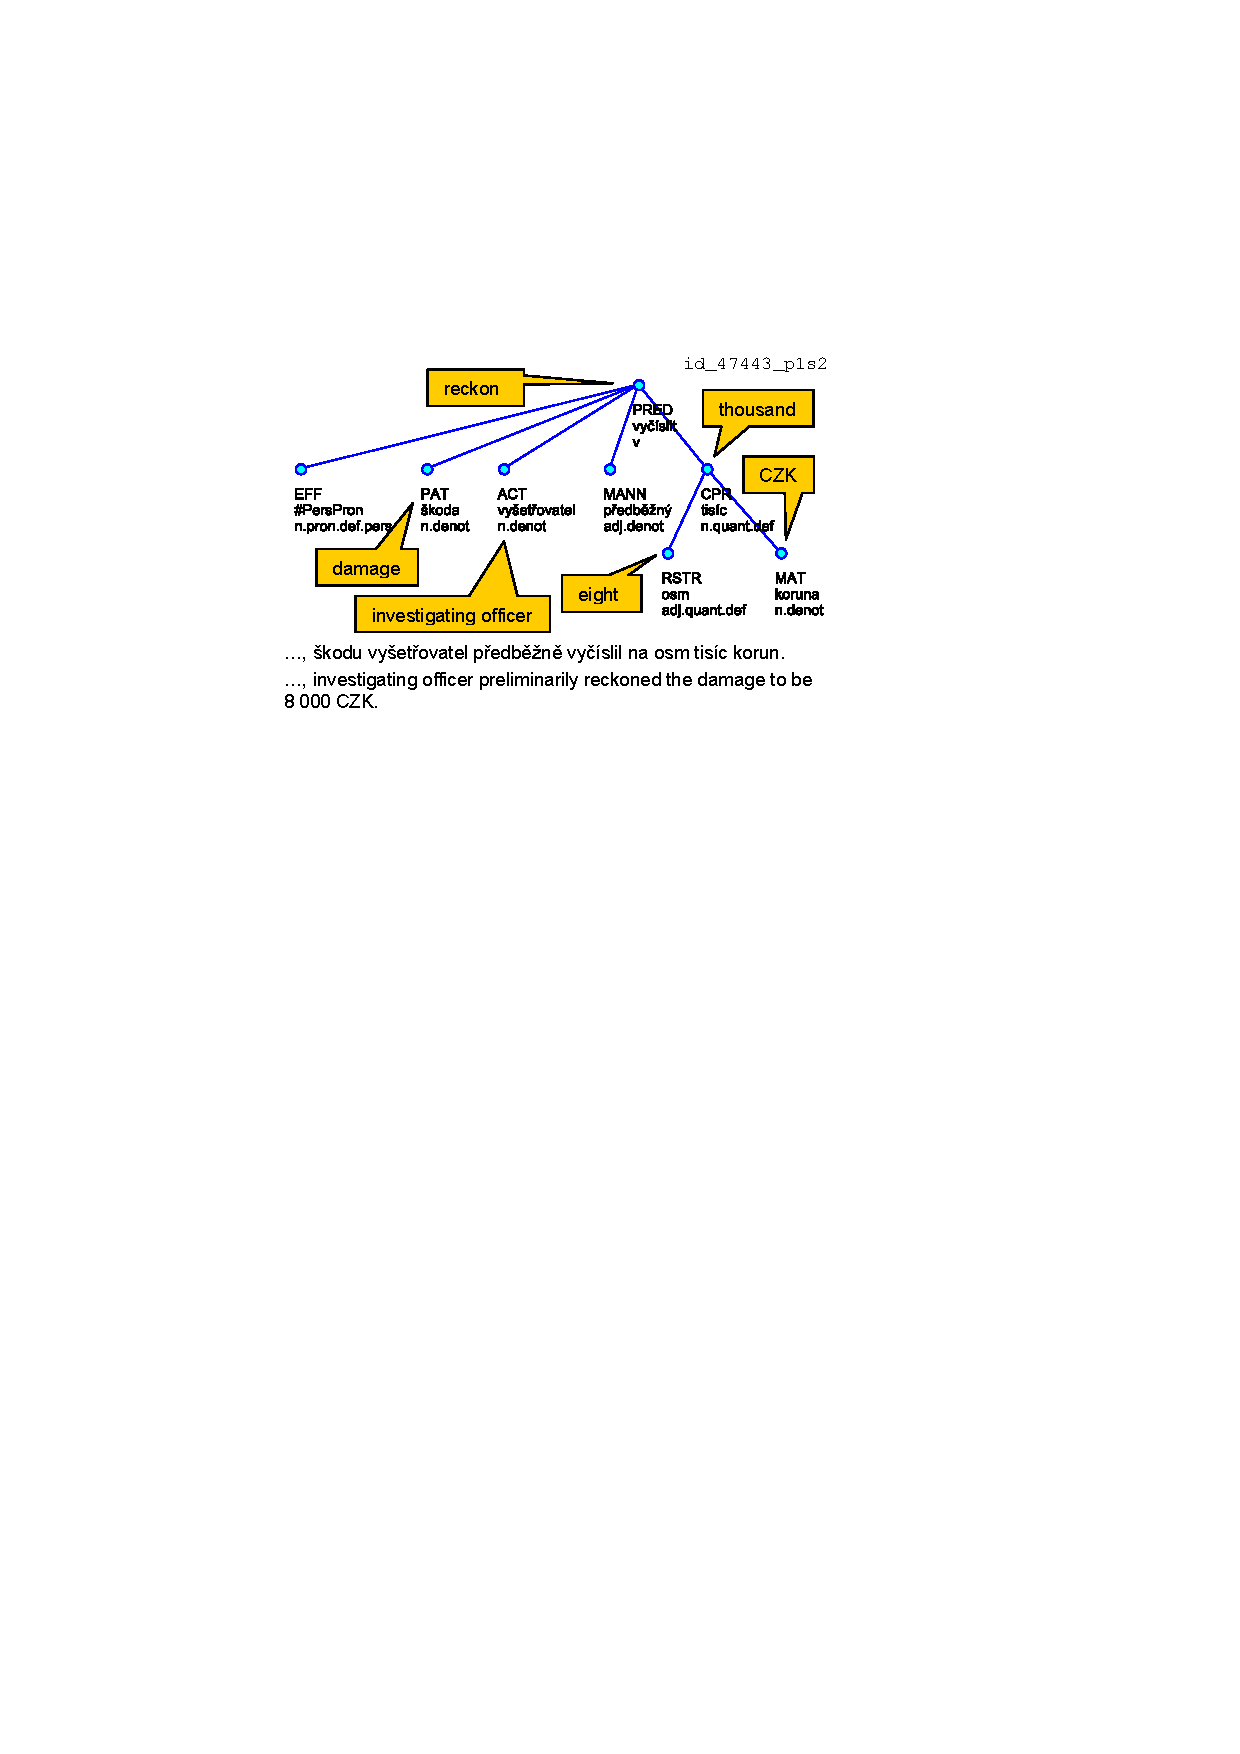
\includegraphics[width=0.55\hsize]{damage_tree}}}
\caption{Example of a linguistic tree of one analyzed sentence.}
\label{img:ch10_damage_tree} 
\end{figure}




%%%%%%%%%%%%%%%%%%%%%%%%%%%%%%%%%%%%%%%%%%%%%%%%%%%%%%%%%%%%%%%%%%%%%%%%%%%%%%%%%%%%%%%%%%
\section{Web Information Extraction Systems for Web Semantization} \label{sec:intro}


There exist many extraction tools that can process web pages and produce structured machine understandable data (or information) that corresponds with the content of a web page. This process is often called Web Information Extraction (WIE). 


In this chapter we present a survey of web information extraction systems and we connect these systems with the problem of web semantization.

The chapter is structured as follows. First we sketch the basic ideas of semantic web and web semantization. In the next two sections methods of web information extraction will presented. Then description of our solutions (work in progress) will continue. And finally just before the conclusion we will discuss the connection of WIE systems with the problem of web semantization.


\subsection{The Semantic Web in Use}



\begin{figure}
\centering
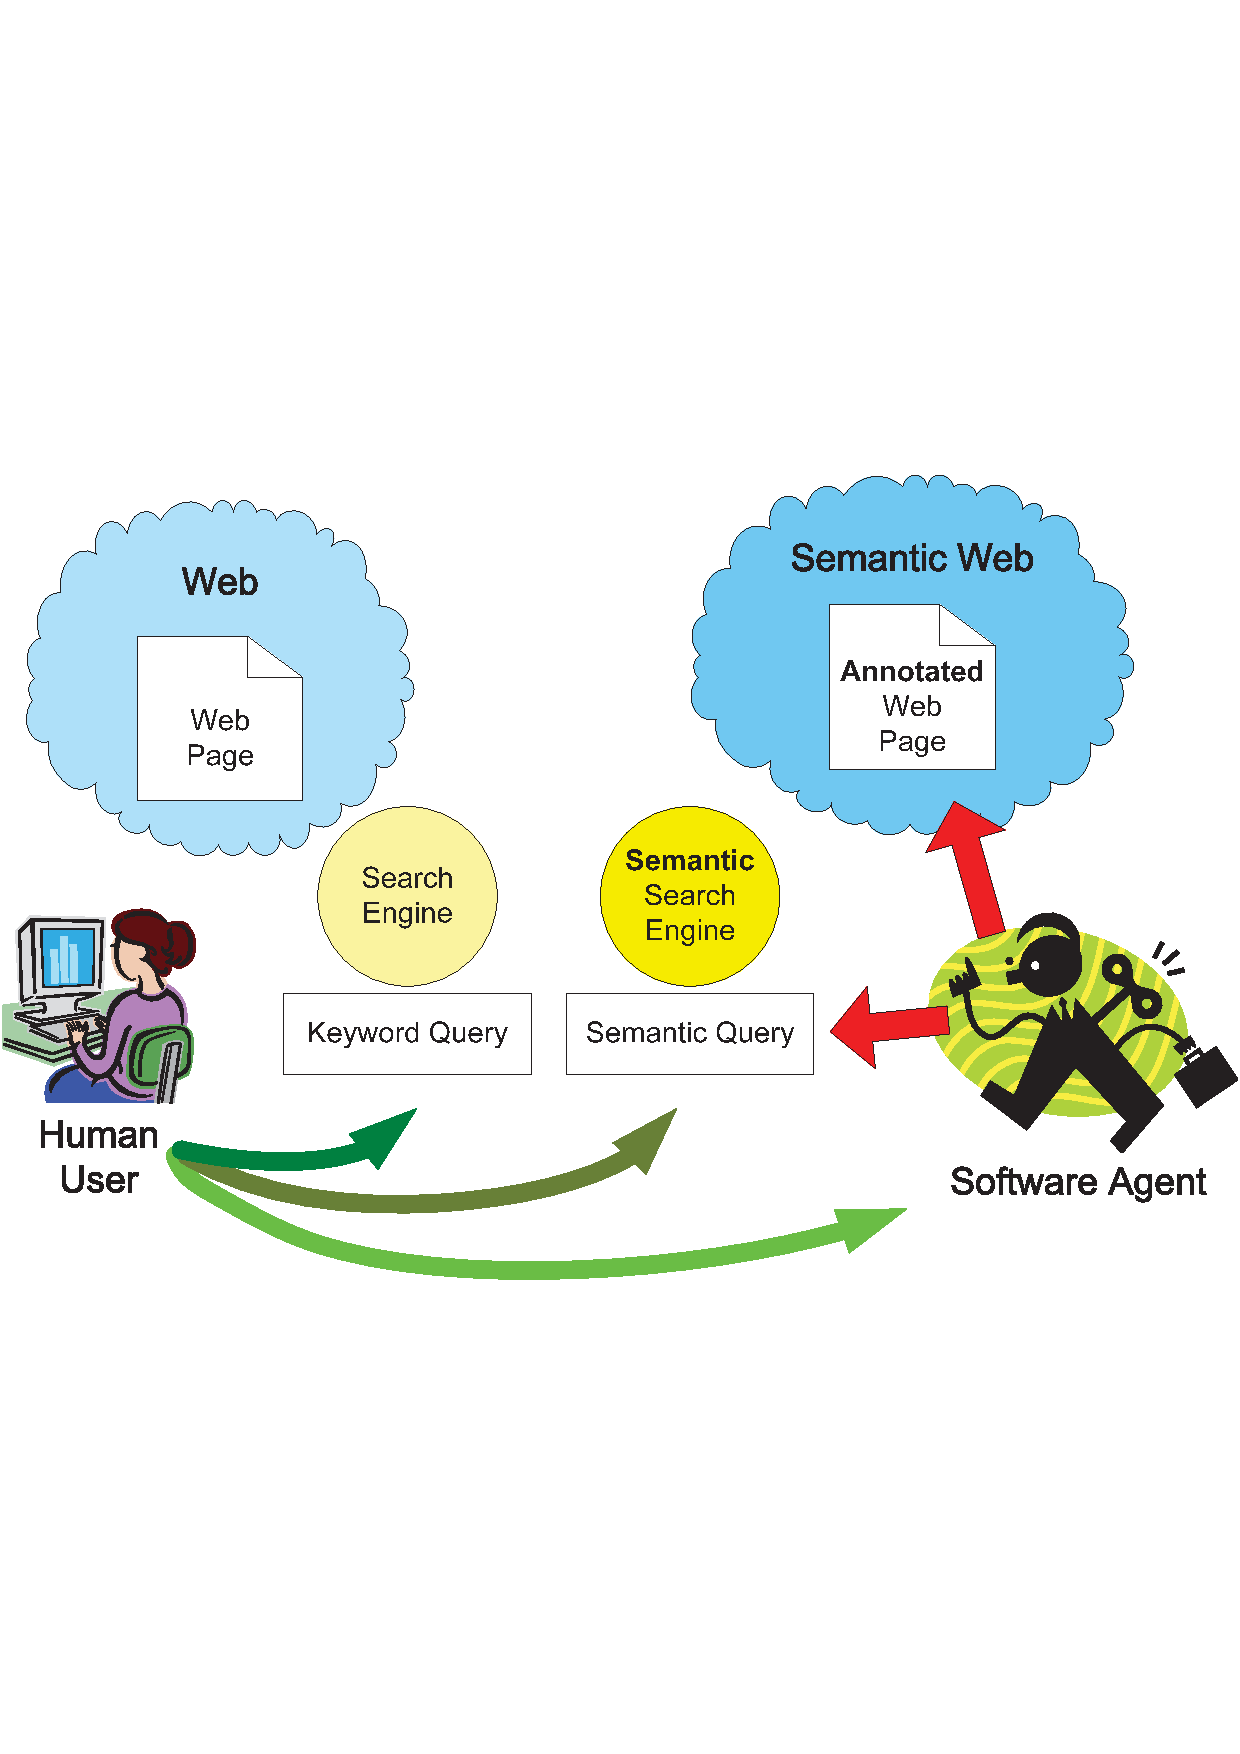
\includegraphics[width=0.6\hsize]{SemanticWeb}
\caption{The Semantic/Semantized Web in Use}
\label{img:SemWebUse}
\end{figure}

The idea of the Semantic Web \citep{biblio:2001-Berners-Lee-SemanticWeb} (World Wide Web dedicated not only to human but also to machine -- software agents) is very well known today. Let us just shortly demonstrate its use with respect to the idea of Web Semantization (see in next section).

The Figure~\ref{img:SemWebUse} shows a human user using the (Semantic) Web in three manners: a keyword query, a semantic query and by using a software agent. The difference between the first two manners (keyword and semantic query) can be illustrated with the question: ``Give me a list of the names of E.U. heads of state.'' This example from interesting article \citep{biblio:Horrocks_Onto} by Ian Horrocks shows the big difference between use of a semantic query language instead of keywords. In the semantic case you should be given exactly the list of names you were requesting without having to pore through results of (probably more then one) keyword queries. Of course the user have to know the syntax of the semantic query language or a special GUI\footnote{Such handy GUI can be found for example in the KIM project \citep{biblio:KIM}.} must be provided.

The last and the most important possibility (in the semantic or semantized setting) is to use some (personalized) software agent that is specialized to tasks of some kind like planning a business trip or finding the most optimal choice from all the relevant job offers, flats for rent, cars for sale, etc.

Both the semantic querying and software agents engagement is impossible without some kind of adaptation of the web of today in the semantic direction. 




\begin{figure}
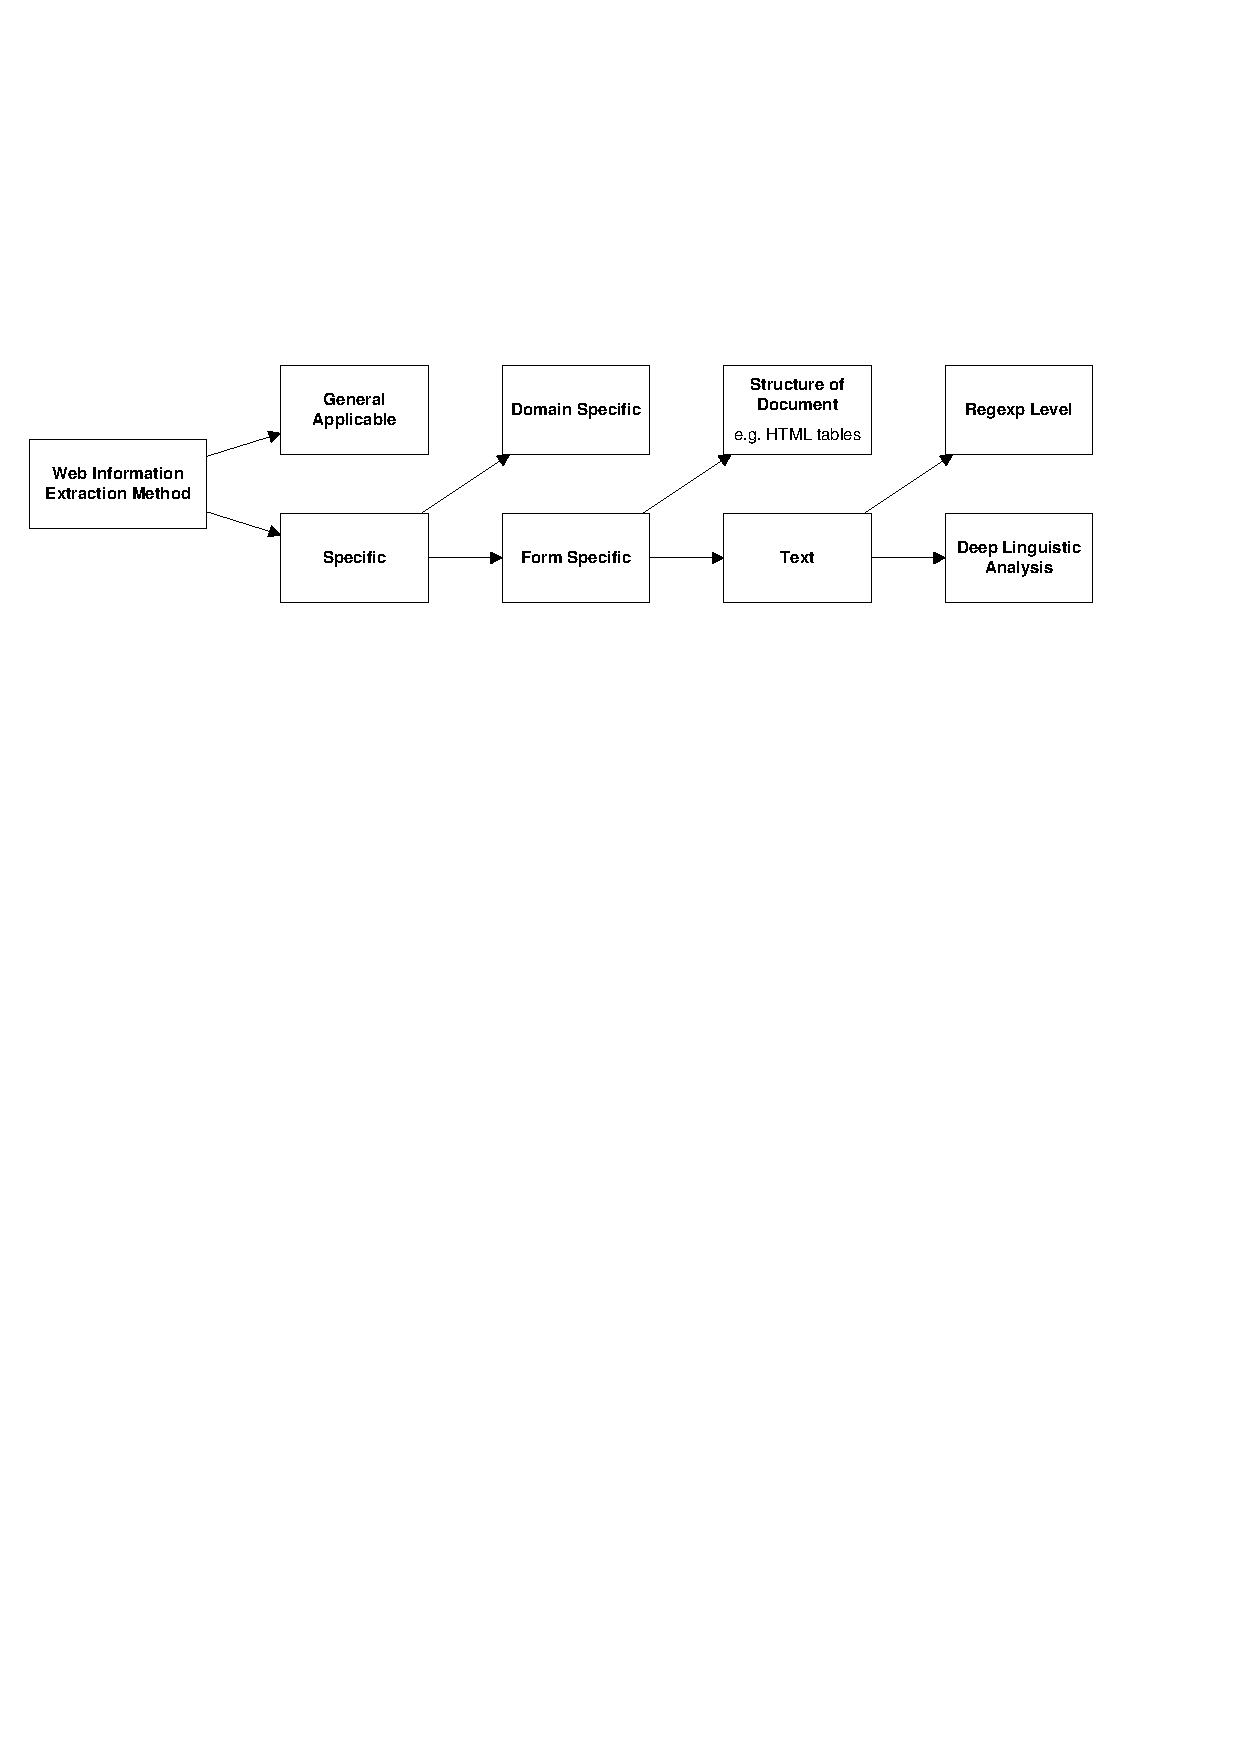
\includegraphics[width=\hsize]{extraction_method}
\caption{Division of extraction methods}
\label{img:extraction_method}
\end{figure}




\subsection{Web Semantization}
The idea of Web Semantization \citep{biblio:DeEcSemantickyWeb2008} consist in gradual enrichment of the current web content as an automated process of third party annotation tools making at least a part of today's web more suitable for machine processing and hence enabling it intelligent tools for searching and recommending things on the web (see \citep{biblio:LeeWebThings}).

The most strait forward idea is to fill a semantic repository with some information that is automatically extracted from the web and make it available to software agents so they could access to the web of today in a semantic manner (e.g. through semantic search engine).

The idea of a semantic repository and a public service providing semantic annotations was experimentally realized in the very recognized work of IBM Almaden Research Center: the SemTag \citep{biblio:seekerIBM}. This work demonstrated that an automated semantic annotation can be applied in a large scale. In their experiment they annotated about 264 million web pages and generated about 434 millions of semantic tags. They also provided the annotations as a \emph{Semantic Label Bureau} -- a HTTP server providing annotations for web documents of 3rd parties.


%%%%%%%%%%%%%%%%%%%%%%%%%%%%%%%%%%%%%%%%%%%%%%%%%%%%%%%%%%%%%%%%%%%%%%%%%%%%%%%%%%%%%%%%%%
\section{Web Information Extraction} \label{sec:WIE}

The task of a web information extraction system is to transform web pages into machine-friendly structures such as relational databases. There exists a rich variety of Web Information Extraction systems. The results generated by distinct tools usually can not be directly compared since the addressed extraction tasks are different. The extraction tasks can be distinguished according several dimensions: domain specificity, automation degree, techniques used, etc. These dimensions are analyzed in detail in the recent publications  \citep{biblio:Chang2006} and \citep{biblio:WebDataMining}. Here we will concentrate on a little bit more specific division of WIE according to the needs of the Web Semantization (see in Sect.~\ref{sec:SemantizationSetting}). The division is demonstrated on the Figure~\ref{img:extraction_method} and should not be considered as disjoint division of the methods but rather as emphasizing different aspects of the methods. For example many extraction methods are domain and form specific at the same time.

The distinguishing between general applicable methods and the others that have meaningful application only in some specific setting (specific domain, specific form of input) is very important for Web Semantization because when we try to produce annotations in large scale, we have to control which web resource is suitable for which processing method (see in Sect.~\ref{sec:SemantizationSetting}). 

%specificke - tez vsude pouzitelne, ale nic nenajdou


\subsection{General Applicable}
The most significant (and probably the only one) generally applicable IE task is so called \emph{Instance Resolution Task}. The task can be described as follows: Given a general ontology, find all the instances from the ontology that are present in the processed resource. This task is usually realized in two steps: (1) Named Entity Recognition (see in Sect.~\ref{sec:LingIETasks}), (2) Disambiguation of ontology instances that can be connected with the found named entities. Success of the method can be strongly improved with coreference resolution (see in Sect.~\ref{sec:LingIETasks}).

Let us mention several good representatives of this approach: the SemTag application \citep{biblio:seekerIBM}, the KIM project \citep{biblio:KIM} and the PANKOW annotation method \citep{biblio:SelfAnnotWeb} based on smart formulation of Google API queries.


\subsection{Domain Specific}

Domain and from specific IE approaches are the typical cases. More specific information is more precise, more complex and so more useful and interesting. But the extraction method has to be trained to each new domain separately. This usually means indispensable effort.

A good example of domain specific information extraction system is SOBA \citep{biblio:SOBA}. This complex system is capable to integrate different IE approaches and extract information from heterogeneous data resources, including plain text, tables and image captions but the whole system is concentrated on the single domain of football. Next similarly complex system is ArtEquAKT \citep{biblio:ArtEquAKT}, which is entirely concentrated on the domain of art.

\subsection{Form Specific}

Beyond general applicable extraction methods there exist many methods that exploit specific form of the input resource. The linguistic approaches usually process text consisting of natural language sentences. The structure-oriented approaches can be strictly oriented on tables \citep{biblio:tables} or exploit repetitions of structural patterns on the web page \citep{biblio:repetitons} (such algorithm can be only applicable
to pages that contain more than one data record), and there are also approaches that use the structure of whole site (e.g. site of single web shop with summary pages with products connected with links to pages with details about single product) \citep{biblio:extraction_detail_pages}. 



%\subsection{Alternative Solutions}

%wikipedia

%hodnoceni - tez velmi relevantni k semantickemu webu



%%%%%%%%%%%%%%%%%%%%%%%%%%%%%%%%%%%%%%%%%%%%%%%%%%%%%%%%%%%%%%%%%%%%%%%%%%%%%%%%%%%%%%%%%%
\section{Information Extraction from Text-based Resources} \label{sec:LingIE}
In this section we will discuss the information extraction from textual resources.

\subsection{Tasks of Information Extraction} \label{sec:LingIETasks}
There are classical tasks of text preprocessing and linguistic analysis like 
\begin{description}
	\item[Text Extraction] -- e.g from HTML, PDF or DOC,
	\item[Tokenization] -- detection of words, spaces, punctuations, etc.,
	\item[Segmentation] -- sentence and paragraph detection,
	\item[POS Tagging] -- part of speech assignment, often including lemmatization and morphological analysis,
	\item[Syntactic Analysis] (often called linguistic \emph{parsing}) -- assignment of the grammatical structure to given sentence with respect to given linguistic formalism (e.g. formal grammar),
	\item[Coreference Resolution] (or \emph{anaphora resolution}) -- resolving what a pronoun, or a noun phrase refers to. These references often cross boundaries of a single sentence.
\end{description}

\noindent Besides these classical general applicable tasks, there are further well defined tasks, which are more closely related to the information extraction. These tasks are domain dependent. These tasks were widely developed in the MUC-6 conference 1995 \citep{biblio:MUC6} and considered as semantic evaluation in the first place. These information extraction tasks are:

\begin{description}
	\item[Named Entity Recognition:] This task recognizes and classifies named entities such as persons, locations, date or time expression, or measuring units. More complex patterns may also be recognized as structured entities such as addresses.
	\item[Template Element Construction:] Populates templates describing entities with extracted
roles (or attributes) about one single entity. This task is often performed stepwise sentence by sentence, which results in a huge set of partially filled templates.
	\item[Template Relation Construction:] As each template describes information about one single entity, this tasks identifies semantic relations between entities.
	\item[Template Unification:] Merges multiple elementary templates that are filled with information about identical entities.
	\item[Scenario Template Production:] Fits the results of Template Element Construction and Template Relation Construction into templates describing pre-specified event scenarios (pre-specified ``queries on the extracted data'').
\end{description}

%Appelt and Israel 
\cite{biblio:Appelt-Israel} wrote an excellent tutorial summarizing these traditional IE tasks and systems built on them.

\subsubsection{Entity Recognition}
\subsubsection{Relation Extraction}
\subsubsection{Event Extraction}


  

\subsection{Information Extraction Benchmarks}

Contrary to the WIE methods based on the web page structure, where we (the authors) do not know about any well established benchmark for these methods\footnote{It is probably at least partially caused by the vital development of the presentation techniques on the web that is still well in progress.}, the situation in the domain of text based IE is fairly different. There are several conferences and events concentrated on the support of automatic machine processing and understanding of human language in text form. Different research topics as text (or information) retrieval\footnote{e.g. Text REtrieval Conference (TREC)\\ \url{http://trec.nist.gov/}}, text summarization\footnote{e.g. Document Understanding Conferences\\ \url{http://duc.nist.gov/}} are involved.

On the filed of information extraction, we have to mention the long tradition of the Message Understanding Conference\footnote{Briefly summarized in \url{http://en.wikipedia.org/wiki/Message_Understanding_Conference}.} \citep{biblio:MUC6} starting in 1987. In 1999 the event of \emph{Automatic Content Extraction (ACE) Evaluation}\footnote{\url{http://www.itl.nist.gov/iad/mig/tests/ace/}} started, which is becoming a track in the Text Analysis Conference (TAC)\footnote{\url{http://www.nist.gov/tac}} this year (in 2009).

All these events prepare several specialized datasets together with information extraction tasks and play an important role as information extraction benchmarks. 

%%%%%%%%%%%%%%%%%%%%%%%%%%%%%%%%%%%%%%%%%%%%%%%%%%%%%%%%%%%%%%%%%%%%%%%%%%%%%%%%%%%%%%%%%%
\section{Our Solutions} \label{sec:OurSolutins}
%\subsection{Extraction Based on Structural Similarity}
%
%Our first approach for the web information extraction is to use the structural similarity in web pages containing large number of table cells and for each cell a link to detailed pages. This is often presented in web shops and on pages that presents more than one object (product offer). Each object is presented in a similar way and this fact can be exploited.
%
%As web pages of web shops are intended for human usage creators have to make their comprehension easier. Acquaintance with several years of web shops has converged to a more or less similar design fashion. There are often cumulative pages with many products in a form of a table with cells containing a brief description and a link to a page with details about each particular product.
%
%Our main idea is to use a DOM tree representation of the summary web page and by breadth first search encounter similar subtrees. The similarity of these subtrees is used to determine the data region -- a place where all the objects are stored. It is represented as a node in the DOM tree, underneath it there are the similar sub-trees, which are called data records.
%
%%Using some heuristics we can detect what are resources described in this page. To~detect possible attributes and even their values we explore similarities between the content of a data record and corresponding content of a detailed page. The main idea is to find same pieces of text in the data record and in the detail page. This occurs often, because a brief summary of the object (e.g. a product) is present in the data record. Somewhere near the attribute values are located the names of attributes in the detail page. These names of attributes can be extracted. The extraction of attribute names is easy because on every detail page the names will be the same.
%
%We\footnote{Thanks go mainly to Du�an Maru�?�k and Peter Vojt�.} have developed and implemented this idea \citep{biblio:EcHoUncertaintyIssues2008} on the top of Mozilla Firefox API and experimentally tested on table pages from several domains (cars, notebooks, hotels). Similarity between subtrees was Levenshtein editing distance (for a subtree considered as a linear string), learning thresholds for decision were trained.
%

\subsection{Linguistic Information Extraction}
Our second approach \citep{biblio:DeVoExploitationlinguistic2008,biblio:DeVoLinguisticextraction2008,biblio:DeVoComputingaggregations2008} for the web information extraction is based on deep linguistic analysis. We have developed a rule-based  method for extraction of information from text-based web resources in Czech and now we are working on its adaptation to English. The extraction rules correspond to tree queries on linguistic (syntactic) trees made form particular sentences. We have experimented with several linguistic tools for Czech, namely Tools for machine annotation -- PDT 2.0 and the Czech WordNet.

Our present system captures text of web-pages, annotates it linguistically by PDT tools, extracts data and stores the data in an ontology. We have made initial experiments in the domain of reports of traffic accidents. The results showed that this method can e.g. aid summarization of the number of injured people.

To avoid the need of manual design of extraction rules we focused on the data extraction phase and made some promising experiments \citep{biblio:DeEcExperimentswith2008} with the machine learning procedure of Inductive Logic Programming for automated learning of the extraction rules.

This solution is directed to extraction of information which is closely connected with the meaning of text or meaning of a sentence. 

%Difficult task.

%Problematic usage of extracted data.


%%%%%%%%%%%%%%%%%%%%%%%%%%%%%%%%%%%%%%%%%%%%%%%%%%%%%%%%%%%%%%%%%%%%%%%%%%%%%%%%%%%%%%%%%%
\section{The Web Semantization Setting} \label{sec:SemantizationSetting}

In this section we will discuss possibilities and obstructions connected with the employment of web information extraction systems in the process of web semantization.

%\subsection{Integration of Extraction Tools}

One aspect of the realization of the web semantization idea is the problem of integration of all the components and technologies starting with web crawling, going through numerous complex analyses (document preprocessing, document classification, different extraction procedures), output data integration and indexing, and finally implementation of query and presentation interface. This elaborate task is neither easy nor simple but today it is solved in all the extensive projects and systems mentioned above.

The novelty that web semantization brings into account is the cross domain aspect. If we do not want to stay with just general ontologies and general applicable extraction methods then we need a methodology how to deal with different domains. The system has to support extension to a new domain in generic way. So we need a methodology and software to support this action. This can for example mean: to add a new ontology for the new domain, to select and train proper extractors and classifiers for the suitable input pages.


\subsection{User Initiative and Effort}
An interesting point is the question: Whose effort will be used in the process of supporting new domain in the web semantization process? How skilled such user has to be? There are two possibilities (demonstrated on the Fig~\ref{img:extraction_proces_and_user}). The easier one is that we have to employ very experienced expert who will decide about the new domain and who will also realize the support needed for the new domain. In the Fig~\ref{img:extraction_proces_and_user} this situation is labeled as \emph{Provider Initiated} and \emph{Provider Trained} because the expert works on the side of the system that provides the semantics. 

\begin{figure}
\centering
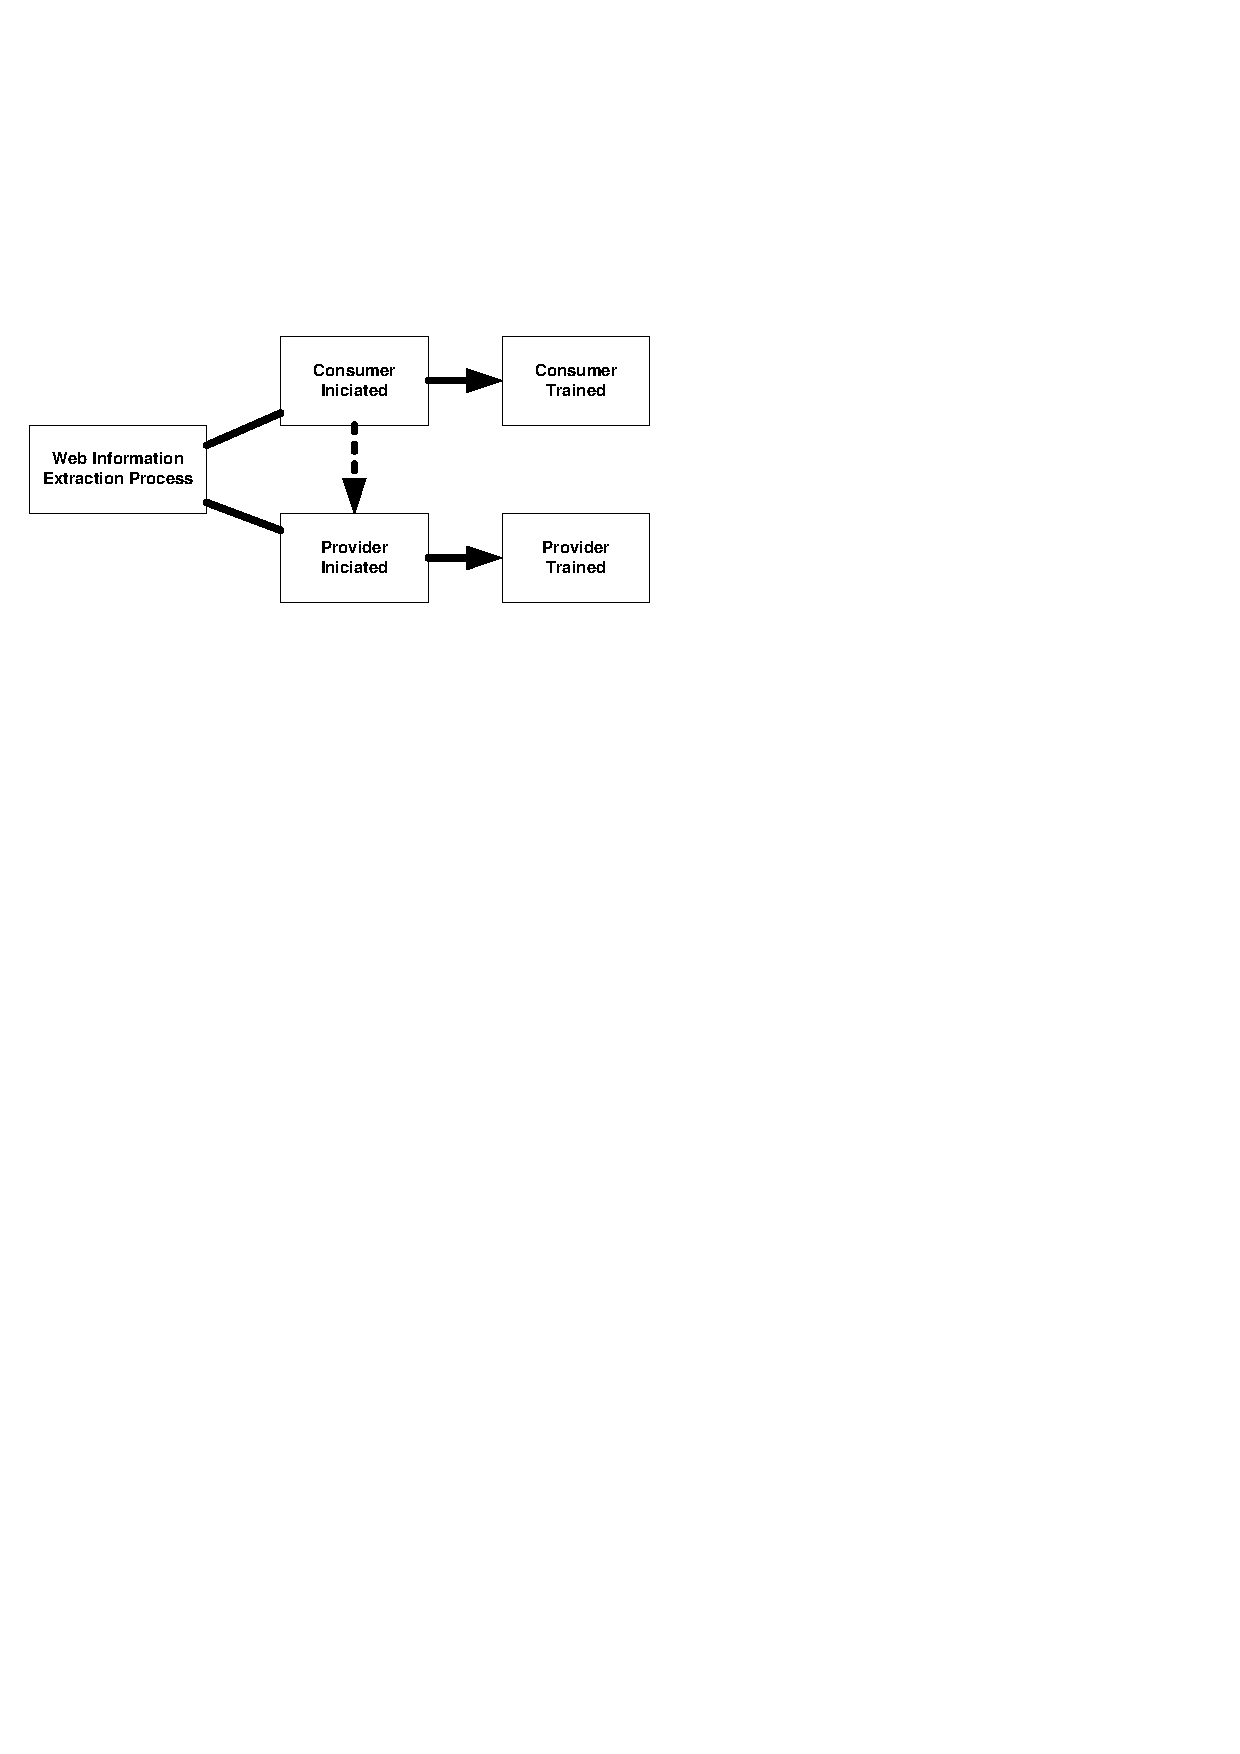
\includegraphics[width=0.6\hsize]{extraction_proces_and_user}
\caption{User initiative and effort}
\label{img:extraction_proces_and_user}
\end{figure}

The second possibility is to enable ordinary users form outside to add a new domain to the semantization system. Such user is probably interested in semantic data form the domain so we call such user \emph{Consumer}.

A cooperation of a consumer (possibly a domain expert) and a provider (system expert) on the support of the new domain can be considered as hybrid approach. This is represented with the dashed arrow in the Fig~\ref{img:extraction_proces_and_user}.

%%%%%%%%%%%%%%%%%%%%%%%%%%%%%%%%%%%%%%%%%%%%%%%%%%%%%%%%%%%%%%%%%%%%%%%%%%%%%%%%%%%%%%%%%%
\section{Conclusion and Future Work} \label{sec:conlusion}

In this chapter we tried to show the complexity of the problem of web semantization in connection with the possibilities of web information extraction systems. Future work goes in several directions: 
\begin{itemize}
	\item Future development of WIE tools and work on their adaptability to new domains.
	\item Integration of WIE tools to the web semantization system.
	\item Development of the methodology and software to support the extension of the semantization system to a new domain for a non-expert user.
\end{itemize}
